\subsection{Ёмкостные акселерометры}
Принцип работы ёмкостных акселерометров основан на изменении емкости конденсаторов при изменении ускорения.

\begin{figure}[ht]
	\centering
	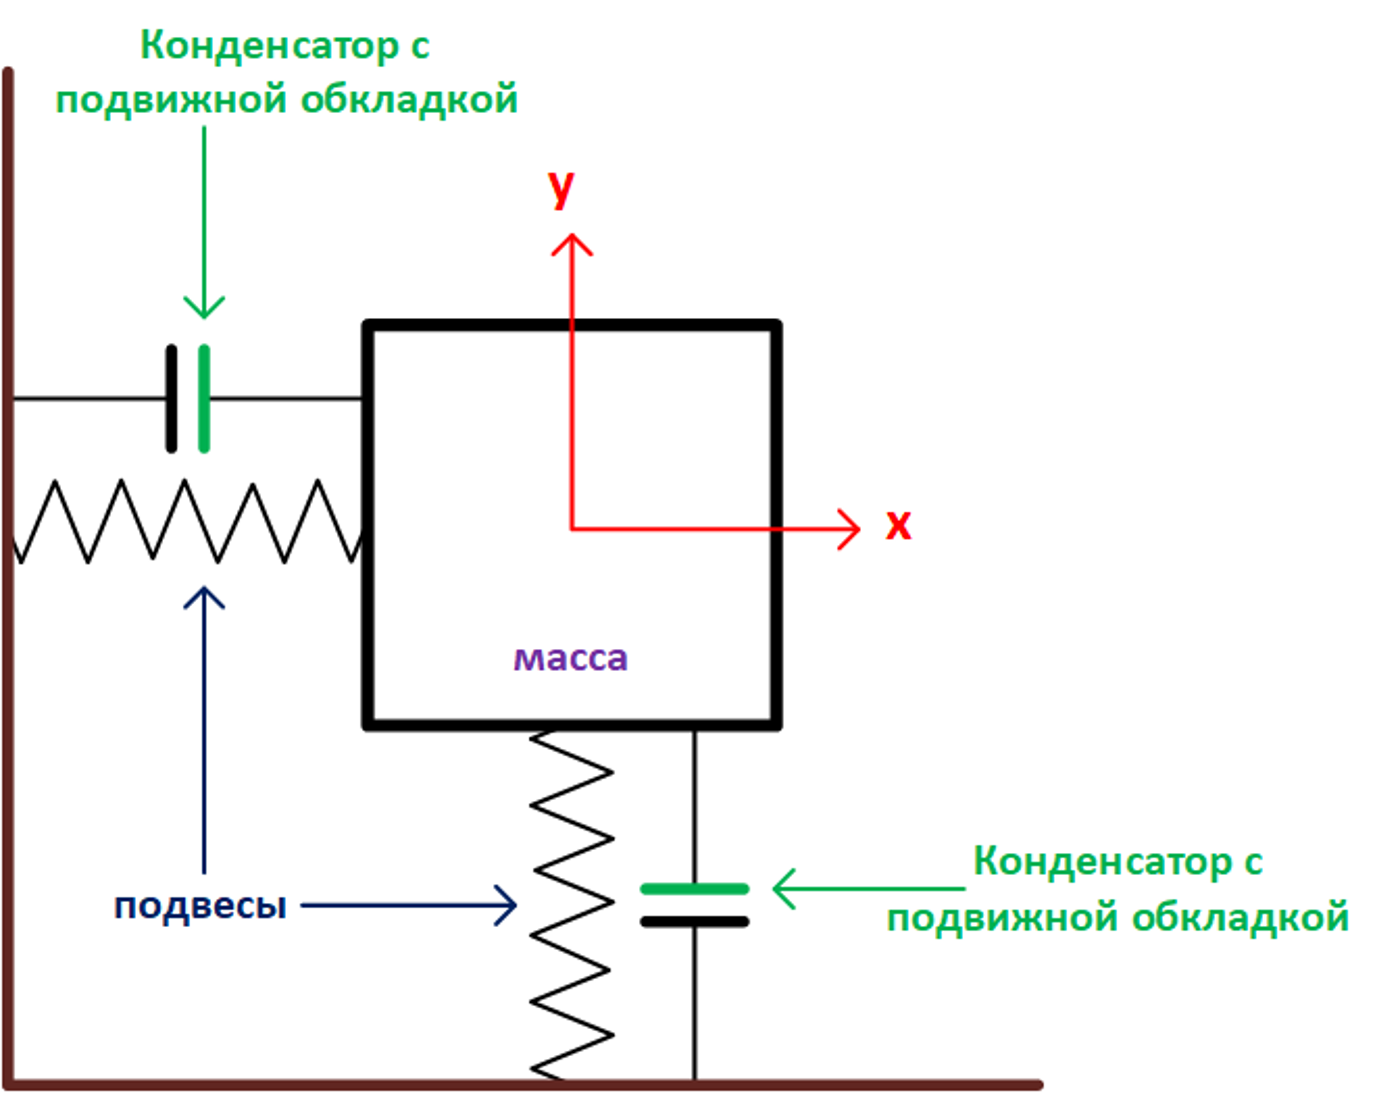
\includegraphics[width=0.55\textwidth]{images/theory/акселерометры/Схема ёмкостного акселерометра.png}
	\caption{Простейшая схема ёмкостного акселерометра}
\end{figure}

При изменении ускорения, масса изменяет расстояние между обкладками конденсатора. Из простейшей формулы емкости конденасатора $C=\frac{\varepsilon\varepsilon_0S}{d} $ следует, что при изменении d расстояния между обкладками емкость конденсатора будет также изменяться. \\ 

\begin{figure}[ht]
	\centering
	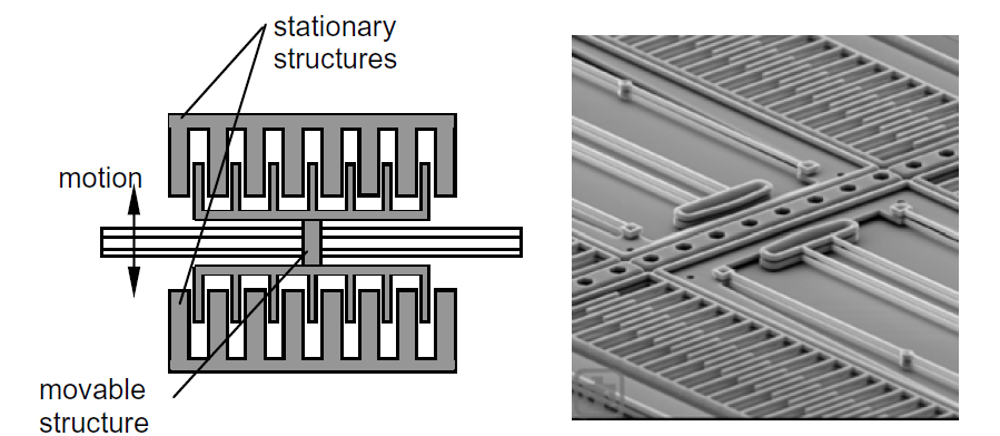
\includegraphics[width=0.7\textwidth]{images/theory/акселерометры/Изображение ёмкостного датчика.png}
	\caption{Устройство ёмкостного акселерометра, выполненного на кремниевой подложке}
\end{figure}

Изменение ёмкости превращается в сигнал с помощью довольно распространённой схемы - ёмкостной полумост.

\begin{figure}[ht]
	\centering
	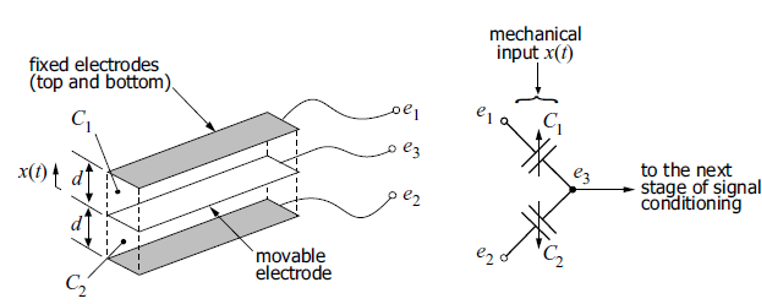
\includegraphics[width=0.7\textwidth]{images/theory/акселерометры/Схема ёмкостного полумоста.png}
	\caption{Схема ёмкостного полумоста}
\end{figure}

Напряжения $e_1$ и $e_2$ являются входными, а $e_3$ – выходной сигнал для последующего преобразования. Емкости обоих конденсаторов зависят от внешнего ускорения, и изменяются на величину x(t). При x = 0, заряды на емкостях являются идентичными, и при этом $C_1=C_2=C_0$. При условии, что x << d найдем как зависит изменение емкости конденсаторов от изменения положения обкладки.

Запишем изменение каждой емкости при сдвиге обкладки на x:
\begin{equation*}
	\Delta C_1=C_1-C_0 \ \ \ \ \ \ \ \ \ \ \ \ \ \  
	\Delta C_2=-C_2+C_0
\end{equation*}


Запишем через формулу емкости:
\begin{equation*}
	\Delta C_1=\frac{\varepsilon S}{d-x}-\frac{\varepsilon S}{d} \ \ \ \ \ \ \ \ \ \ \ \ \ \ \
	\Delta C_2=-\frac{\varepsilon S}{d+x}+\frac{\varepsilon S}{d}
\end{equation*}


Упростим данные формулы и учтём, что x << d. Тогда получим формулу изменения емкости конденсатора, в зависимости от смещения обкладки:
\begin{equation*}
	\Delta C_1=\frac{\varepsilon Sx}{d^2-xd}; \ \ \ \ \ \ 
	\Delta C_2=\frac{\varepsilon Sx}{d^2+xd} \\
\end{equation*}

\begin{equation}
	\Delta C\left(x\right)=\frac{\varepsilon S}{d^2}x
\end{equation}

\hspace{0.5cm}

Вводём дополнительные токи — $i_1, i_2, i_3$. По первому закону Киргофа получаем $i_1 + i_2 = i_3$ \\ 
Учитывая тот факт, что ток является производной заряда $i = \frac{dq}{dt}$ и заряд \ \ $q=CU$, получаем при $e_1=e_s$, а $e_2=-e_s$ зависимость выходного тока:

\begin{equation}
	i_{3} = 2 \left( e_{s} \frac{\epsilon S}{d^2} \dot{x} + x \frac{\epsilon S}{d^2} \dot{e_{s}} - C_{0}\dot{e_{s}} \right) 
\end{equation}

\newpage